\documentclass[a4paper,oneside]{book}
\usepackage{listings}
\usepackage{amsmath}
\usepackage{listings}
\usepackage{epsfig}
\usepackage{color}
\definecolor{grayLines}{gray}{0.6}
\definecolor{grayText}{gray}{0.3}
\usepackage{multirow}
\usepackage{wasysym}
\usepackage{gensymb} 

\begin{document}
\lstset{language=Python}          % Set your language (you can change the language for each code-block optionally)
\setcounter{secnumdepth}{3}
\setcounter{tocdepth}{3}
\tableofcontents

\chapter{Finite element model components}

\section{Nodes}

\subsection{Description}
The nodes of a finite element mesh are the points where the degrees of freedom reside. Each node object has, at least, the following information:

\begin{itemize}
\item Coordinates wich define its position in space. Typically (x,y,z) coordinates.
\item Definition of the degrees of freedom in the node (displacements, rotations,\ldots)
\end{itemize}

The nodes can also serve to define loads or masses that act over the model at its position.

\subsection{Node creation}

To create a node you can use the following commands:

\begin{lstlisting}[frame=single]
  nodos.newNodeXY(x,y)
  nodos.newNodeIDXY(tag,x,y)
  nodos.newNodeXYZ(x,y,z)
  nodos.newNodeIDXYZ(x,y,z)
\end{lstlisting}

\noindent where:

\begin{description}
\item{nodos:} is a node container obtained from the preprocessor.
\item{tag:} is an integer that identifies the node in the model.
\item{(x,y) or (x,y,z):} are the cartesian coordinates that define node's position.
\end{description}

\subsection{Predefined spaces}
Nodes definition in typical elastic FE models.
\begin{verbatim}
from model import predefined_spaces as ps
nodos= preprocessor.getNodeLoader
\end{verbatim}
\begin{center} 
\begin{longtable}{ll}
{\tt ps.gdls\_elasticidad2D(nodos)} & 2 node coordinates $(x,y)$ \\
                                    & 2 node DOF $(u_x,u_y)$ \\ 
{\tt ps.gdls\_resist\_materiales2D(nodos)} & 2 node coordinates $(x,y)$ \\
                                    & 3 node DOF $(u_x,u_y,\theta)$ \\ 
{\tt ps.gdls\_elasticidad3D(nodos)} & 3 node coordinates $(x,y,z)$ \\
                                    & 3 node DOF $(u_x,u_y,u_z)$ \\ 
{\tt ps.gdls\_resist\_materiales3D(nodos)} & 3 node coordinates $(x,y)$ \\
                                    & 6 node DOF $(u_x,u_y,u_z,\theta_x,\theta_y,\theta_z)$ \\ 
\end{longtable} \end{center}



\section{Constraints}
\subsection{MP constraints}

\subsubsection{Description}
An MP\_Constraint represents a multiple point constraint in the domain. A multiple point constraint imposes a relationship between the displacement for certain dof at two nodes in the model, typically called the {\em retained} node and the {\em constrained} node:

\begin{equation}
U_c = C_{cr} U_r
\end{equation}


An MP\_Constraint is responsible for providing information on the relationship between the dof, this is in the form of a constraint matrix, $C_{cr}$, and two ID objects, {\em retainedID} and {\em constrainedID} indicating the dof's at the nodes represented by $C_{cr}$. For example, for the following constraint imposing a relationship between the displacements at node $1$, the constrained node, with the displacements at node $2$, the retainednode in a problem where the x,y,z components are identified as the 0,1,2 degrees-of-freedom:

\begin{align}
u_{1,x} &= 2 u_{2,x} + u_{2,z} \\
u_{1,y} &= 3 u_{2,z}
\end{align}

\noindent the constraint matrix is:

\begin{equation}
C_{cr} =
\left[
\begin{array}{cc}
2 & 1  \\
0 & 3
\end{array}
\right] 
\end{equation}

\noindent and the vectors defining the dof's at the nodes are:

\begin{align}
constrainedID &= [0, 1] \\
retainedID &= [0, 2]
\end{align}



\chapter{Solver components}

\section{Analysis components}
\subsection{Constraints}

\subsubsection{LagrangeMP\_FE}
LagrangeMP\_FE is a subclass of FE\_Element used to enforce a
multi point constraint, of the form $U_c = C_{cr} U_r$, where $U_c$ are
the constrained degrees-of-freedom at the constrained node, $U_r$ are
the retained degrees-of-freedom at the retained node and $C_{cr}$ a
matrix defining the relationship between these degrees-of-freedom. 

To enforce the constraint the following are added to the tangent and
the residual:
\[ \left[ \begin{array}{cc} 0 & \alpha C^t \\ \alpha C & 0 \end{array}
\right] ,
\left\{ \begin{array}{c} 0 \\ 0 \end{array} \right\} \]

\noindent at the locations
corresponding to the constrained degree-of-freedoms specified by the
MP\_Constraint, i.e. $[U_c$ $U_r]$, and the lagrange multiplier
degrees-of-freedom introduced by the LagrangeConstraintHandler for
this constraint, $C = [-I$ $ C_{cr}]$. Nothing is added to the residual. \\  


To construct a LagrangeMP\_FE element to enforce the constraint
specified by the MP\_Constraint {\em theMP} using a default value for
$\alpha$ of $alpha$. The FE\_Element class constructor is called with
the integers $3$ and the two times the size of the {\em retainedID}
plus the size of the {\em constrainedID} at the MP\_Constraint {\em
theMP} plus . A Matrix and a Vector object are created for adding the
contributions to the tangent and the residual. The residual is
zeroed. If the MP\_Constraint is not time varying, then the contribution to the
tangent is determined. Links are set to the retained and constrained
nodes. The DOF\_Group tag ID is set using the tag of the constrained
Nodes DOF\_Group, the tag of the retained Node Dof\_group and the tag
of the LagrangeDOF\_Group, {\em theGroup}. A warning message is printed and 
the program is terminated if either not enough memory is available for
the Matrices and Vector or the constrained and retained Nodes of their
DOF\_Groups do not exist. \\




\indent {\em virtual void setID(void);} \\
Causes the LagrangeMP\_FE to determine the mapping between it's equation
numbers and the degrees-of-freedom. This information is obtained by
using the mapping information at the DOF\_Group objects associated with
the constrained and retained nodes and the LagrangeDOF\_Group, {\em
theGroup}. Returns $0$ if
successful. Prints a warning message and returns a negative number if
an error occurs: $-2$ if the
Node has no associated DOF\_Group, $-3$ if the constrained DOF
specified is invalid for this Node (sets corresponding ID component to
$-1$ so nothing is added to the tangent) and $-4$ if the ID in the
DOF\_Group is too small for the Node (again setting corresponding ID
component to $-1$). \\ 

\indent {\em virtual const Matrix \&getTangent(Integrator *theIntegrator);} \\
If the MP\_Constraint is time-varying, from the MP\_Constraint
{\em theMP} it obtains the current $C_{cr}$ matrix; it then adds the
contribution to the tangent matrix. Returns this tangent Matrix.

\indent {\em virtual const Vector \&getResidual(Integrator *theIntegrator);} \\
Returns the residual, a $zero$ Vector. \\




\chapter{Materials and sections}
\section{Stardard uniaxial materials}
\subsection{defElasticMaterial}
\noindent Construct an elastic uniaxial material
\begin{verbatim}
defElasticMaterial(mdlr,name,E)
\end{verbatim}
\vspace{-10pt}
{\color{grayLines} \rule{\linewidth}{0.25pt}}
\begin{center}
\begin{tabular}{lp{10cm}}
{\tt mdlr} & modeler name \\
{\tt name} & name identifying the material \\
{\tt E} & tangent in the stress-strain diagram (see figure \ref{Elastic}) \\
\end{tabular}
\end{center}
\paragraph{Example}
\begin{verbatim}
*
\end{verbatim}

\begin{figure}[h]
\centering
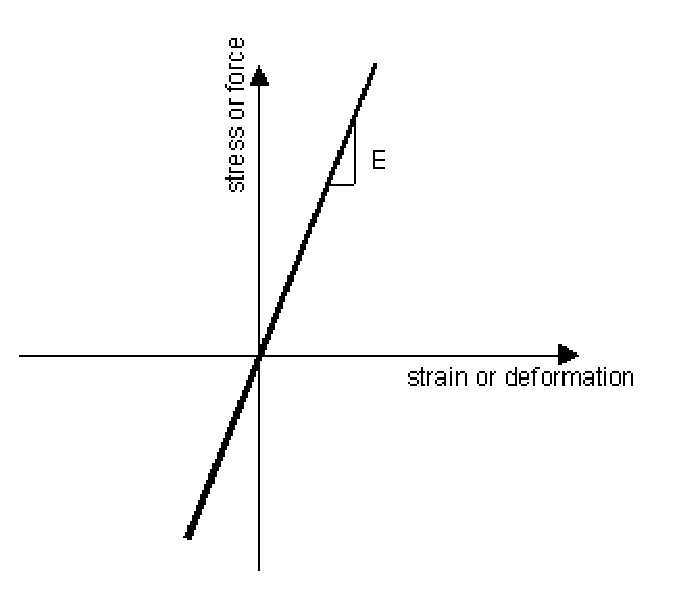
\includegraphics[width=60mm]{materials/figures/Elastic}
\caption{Elastic uniaxial material. Stress-strain diagram}\label{Elastic}
\end{figure}

\subsection{defElasticPPMaterial}
\noindent Construct an elastic perfectly-plastic uniaxial material
\begin{verbatim}
defElasticPPMaterial(mdlr,name,E,fyp,fyn)
\end{verbatim}
\vspace{-10pt}
{\color{grayLines} \rule{\linewidth}{0.25pt}}
\begin{center}
\begin{tabular}{lp{10cm}}
{\tt mdlr} & modeler name \\
{\tt name} & name identifying the material \\
{\tt E} & tangent in the elastic zone of the stress-strain diagram (see figure \ref{ElasticPP}) \\
{\tt fyp} & stress at which material reaches plastic state in tension (see figure \ref{ElasticPP}) \\
{\tt fyn} &  stress at which material reaches plastic state in compression (see figure \ref{ElasticPP}) \\
{\tt } &  \\
\end{tabular}
\end{center}
\paragraph{Example}
\begin{verbatim}
*
\end{verbatim}

\begin{figure}[h]
\centering
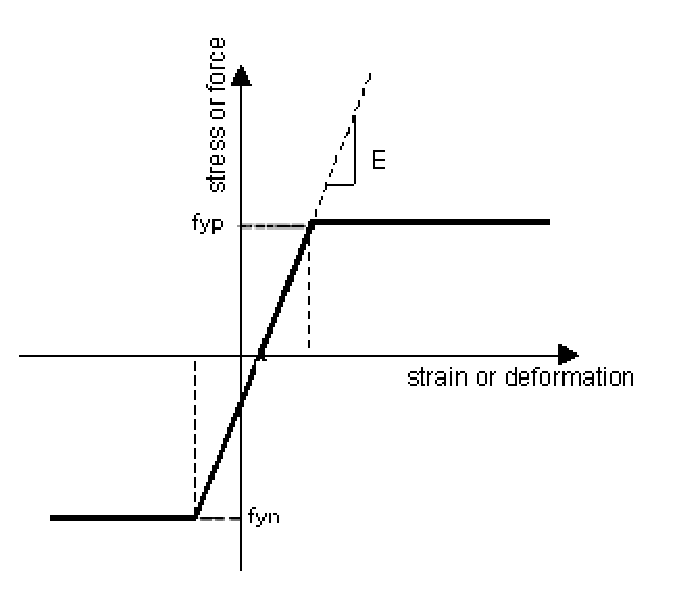
\includegraphics[width=60mm]{materials/figures/ElasticPP}
\caption{Elastic perfectly-plastic uniaxial material. Stress-strain diagram}\label{ElasticPP}
\end{figure}

\subsection{defElastNoTracMaterial}
\noindent Construct a uniaxial elastic-no tension material
\begin{verbatim}
defElastNoTracMaterial(mdlr,name,E)
\end{verbatim}
\vspace{-10pt}
{\color{grayLines} \rule{\linewidth}{0.25pt}}
\begin{center}
\begin{tabular}{lp{10cm}}
{\tt mdlr} & modeler name \\
{\tt name} & name identifying the material \\
{\tt E} & tangent in the elastic zone of the stress-strain diagram (see figure \ref{ENT}) \\
\end{tabular}
\end{center}
\paragraph{Example}
\begin{verbatim}
*
\end{verbatim}
\begin{figure}[h]
\centering
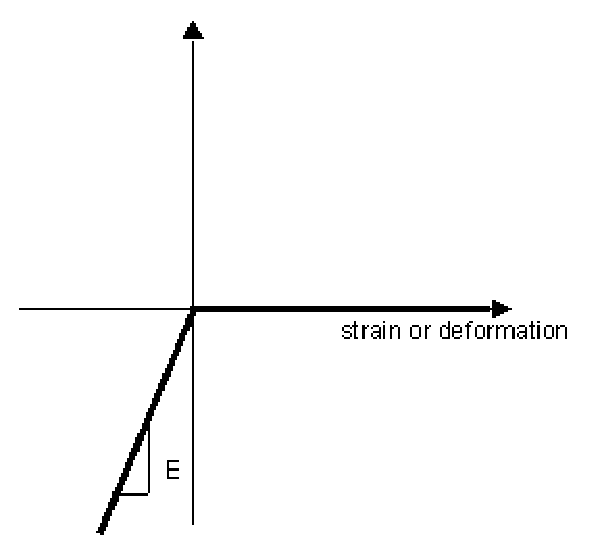
\includegraphics[width=50mm]{materials/figures/ENT}
\caption{Elastic-no tension material. Stress-strain diagram}\label{ENT}
\end{figure}

\section{Steel and reinforcing steel materials}
\subsection{defCableMaterial}
\noindent Construct a uniaxial bilinear prestressed material. The stress strain ranges from slack (large strain at zero stress) to taught (linear with modulus E).
\begin{verbatim}
defCableMaterial(mdlr,name,E,prestress,rho)
\end{verbatim}
\vspace{-10pt}
{\color{grayLines} \rule{\linewidth}{0.25pt}}
\begin{center}
\begin{tabular}{lp{10cm}}
{\tt mdlr} & modeler name \\
{\tt name} & name identifying the material \\
{\tt E} & Young modulus \\
{\tt prestress} & prestress \\
{\tt rho} & effective self weight (gravity component of weight per volume transverse to the cable) \\
\end{tabular}
\end{center}
\paragraph{Example}
\begin{verbatim}
*
\end{verbatim}


\subsection{defSteel01}
\noindent Construct a uniaxial bilinear steel material object with kinematic hardening
\begin{verbatim}
defSteel01(mdlr,name,E,fy,b)
\end{verbatim}
\vspace{-10pt}
{\color{grayLines} \rule{\linewidth}{0.25pt}}
\begin{center}
\begin{tabular}{lp{10cm}}
{\tt mdlr} & modeler name \\
{\tt name} & name identifying the material \\
{\tt E} & initial elastic tangent (see figure \ref{Steel01}) \\
{\tt fy} &  yield strength (see figure \ref{Steel01})\\
{\tt b} &  strain-hardening ratio: ratio between post-yield tangent and initial elastic tangent (see figure \ref{Steel01})\\
\end{tabular}
\end{center}
\paragraph{Example}
\begin{verbatim}
*
\end{verbatim}

\begin{figure}[h]
\centering
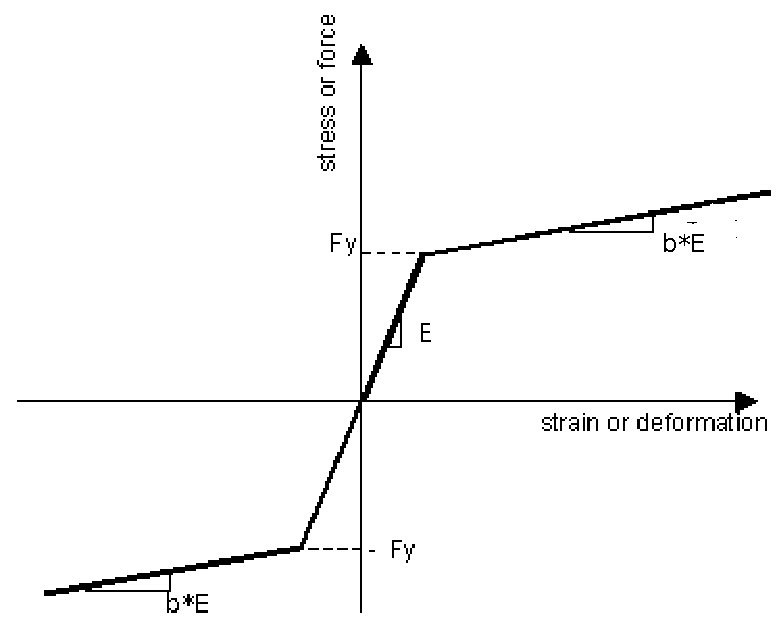
\includegraphics[width=60mm]{materials/figures/Steel01}
\caption{Steel001: uniaxial bilinear steel material with kinematic hardening. Stress-strain diagram}\label{Steel01}
\end{figure}


\subsection{defSteel02}
\noindent Construct a uniaxial Giuffre-Menegotto-Pinto steel material object with isotropic strain hardening
\begin{verbatim}
defSteel02(mdlr,name,E,fy,b,initialStress)
\end{verbatim}
\vspace{-10pt}
{\color{grayLines} \rule{\linewidth}{0.25pt}}
\begin{center}
\begin{tabular}{lp{10cm}}
{\tt mdlr} & modeler name \\
{\tt name} & name identifying the material \\
{\tt E} & initial elastic tangent (see figure \ref{Steel02}) \\
{\tt fy} &  yield strength (see figure \ref{Steel02})\\
{\tt b} &  strain-hardening ratio: ratio between post-yield tangent and initial elastic tangent)\\
{\tt initialStress} &  initial stress \\
\end{tabular}
\end{center}
{\footnotesize The transition from elastic to plastic branches  (see figure \ref{Steel02}) is controlled by parameters R0, R1, R2. The default values R0=15, R1=0.925 and R2=0.15}
\paragraph{Example}
\begin{verbatim}
*
\end{verbatim}

\begin{figure}[h]
\centering
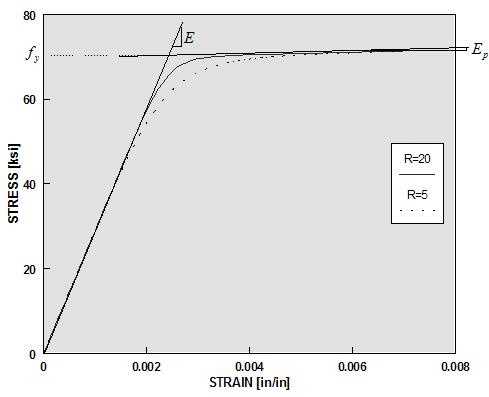
\includegraphics[width=60mm]{materials/figures/Steel02Monotonic}
\caption{Steel002: uniaxial bilinear steel material with isotropic strain hardening. Stress-strain diagram}\label{Steel02}
\end{figure}

\subsection{ReinforcingSteel}
\noindent This class constructs a bilinear stress-strain diagram to carry out the analysis of reinforced concrete according to Eurocode 2. Other national standards, like the spanish EHE and the swiss SIA also adopt this diagram.

\begin{center}
\begin{tabular}{lp{10cm}}
\multicolumn{2}{p{11cm}}{\color{grayText} \large{Parameters}} \\
\multicolumn{2}{p{13cm}}{\color{grayLines} \rule{\linewidth}{0.25pt}} \\
{\tt nmbMaterial} & name identifying the material \\
{\tt nmbDiagK} & name identifying the characteristic stress-strain diagram (default: {\tt "dgK"+nmbMaterial}) \\
{\tt tagDiagK} & tag of the uniaxial material with the characteristic stress-strain diagram\\
{\tt nmbDiagD} &  name identifying the design stress-strain diagram (default: {\tt "dgD"+nmbMaterial}) \\
{\tt tagDiagD} & tag of the uniaxial material with the design stress-strain diagram\\
{\tt fyk} & characteristic value of the yield strength\\
{\tt gammaS} & partial factor for material (default: 1.15)\\
{\tt Es} & elastic modulus of the material (default: 2e11)\\
{\tt emax} & maximum strain at failure point\\
{\tt k} & ratio between characteristic ultimate stress and characteristic yield stress $^{(1)}$ (default: 1.05)\\
\multicolumn{2}{p{13cm}}{\color{grayLines} \rule{\linewidth}{0.25pt}} \\
\multicolumn{2}{p{13cm}}{\footnotesize{(1): according to annex C of EC2: for class A k$\ge$1,05, for class B k$\ge$1,08}}
\end{tabular}
\end{center}

\begin{center}
\begin{tabular}{lp{9cm}}
\multicolumn{2}{p{11cm}}{\color{grayText} \large{Methods}} \\
\multicolumn{2}{p{13cm}}{\color{grayLines} \rule{\linewidth}{0.25pt}} \\
{\tt fmaxk()} & characteristic ultimate strength \\
{\tt fyd()} & design yield stress \\
{\tt eyk()} & characteristic strain at yield point\\
{\tt eyd()} & design strain at yield point\\
{\tt Esh()} &  post-yield tangent\\
{\tt bsh()} & ratio between post-yield tangent and initial elastic tangent\\
{\tt defDiagK(mdlr)} & returns XC uniaxial material (characteristic values)\\
{\tt defDiagD(mdlr)} & returns XC uniaxial material (design values)\\
\end{tabular}
\end{center}

\section{Concrete materials}
\subsection{defConcrete01}
\noindent Construct a uniaxial Kent-Scott-Park concrete material object with degraded linear unloading/reloading stiffness according to the work of Karsan-Jirsa and no tensile strength.
\begin{verbatim}
defConcrete01(mdlr,name,epsc0,fpc,fpcu,epscu)
\end{verbatim}
\vspace{-10pt}
{\color{grayLines} \rule{\linewidth}{0.25pt}}
\begin{center}
\begin{tabular}{lp{10cm}}
{\tt mdlr} & modeler name \\
{\tt name} & name identifying the material \\
{\tt fpc} &  concrete compressive strength at 28 days (compression is negative) $^{(1)}$\\
{\tt epsc0} &  concrete strain at maximum strength (see figure \ref{Concrete01}) $^{(2)}$\\
{\tt fpcu} &  concrete crushing strength (see figure \ref{Concrete01}) \\
{\tt epscu} &  concrete strain at crushing strength (see figure \ref{Concrete01}) \\
\hline
\multicolumn{2}{p{12cm}}{\footnotesize(1): Compressive concrete parameters should be input as negative values (if input as positive, they will be converted to negative internally)}\\
\multicolumn{2}{p{12cm}}{\footnotesize (2): The initial slope for this model is $2*fpc/epsc0$ (see figure \ref{Concrete01})}\\
\end{tabular}
\end{center}
\paragraph{Example}
\begin{verbatim}
*
\end{verbatim}

\begin{figure}[h]
\centering
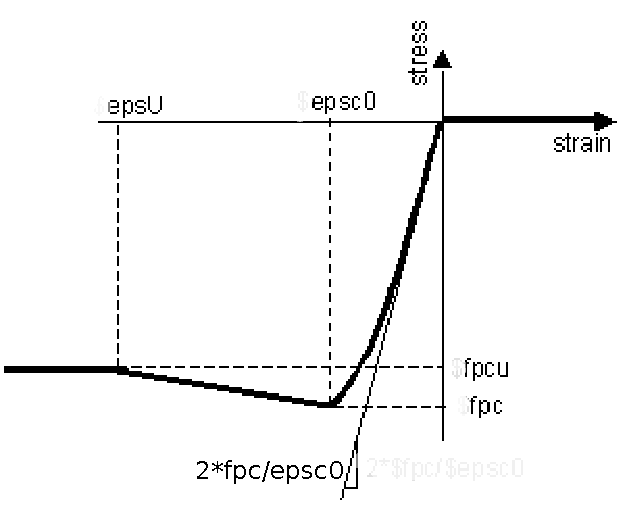
\includegraphics[width=60mm]{materials/figures/Concrete01}
\caption{Concrete01: uniaxial Kent-Scott-Park concrete material. Stress-strain diagram}\label{Concrete01}
\end{figure}

\section{ND materials}
An ND material is an object that represents the stress-strain relationship at the gauss-point of a continuum element.

\subsection{defElasticIsotropic3d}
\noindent Construct an elastic isotropic material.
\begin{verbatim}
defElasticIsotropic3d(mdlr,name,E,nu,rho)
\end{verbatim}
\vspace{-10pt}
{\color{grayLines} \rule{\linewidth}{0.25pt}}
\begin{center}
\begin{tabular}{lp{10cm}}
{\tt mdlr} & modeler name \\
{\tt name} & name identifying the material\\
{\tt E} & elastic modulus \\
{\tt nu} & Poisson's ratio \\
{\tt rho} &  mass density, optional (default = 0.0)\\
\end{tabular}
\end{center}
\paragraph{Example}
\begin{verbatim}
*
\end{verbatim}

\subsection{defElasticIsotropicPlaneStrain}
\noindent Construct an elastic isotropic plane-strain material.
\begin{verbatim}
defElasticIsotropicPlaneStrain(mdlr,name,E,nu,rho)
\end{verbatim}
\vspace{-10pt}
{\color{grayLines} \rule{\linewidth}{0.25pt}}
\begin{center}
\begin{tabular}{lp{10cm}}
{\tt mdlr} & modeler name \\
{\tt name} & name identifying the material\\
{\tt E} & elastic modulus \\
{\tt nu} & Poisson's ratio \\
{\tt rho} &  mass density, optional (default = 0.0)\\
\end{tabular}
\end{center}
\paragraph{Example}
\begin{verbatim}
*
\end{verbatim}

\subsection{defElasticIsotropicPlaneStress}
\noindent Construct an elastic isotropic plane-stress material.
\begin{verbatim}
defElasticIsotropicPlaneStress(mdlr,name,E,nu,rho)
\end{verbatim}
\vspace{-10pt}
{\color{grayLines} \rule{\linewidth}{0.25pt}}
\begin{center}
\begin{tabular}{lp{10cm}}
{\tt mdlr} & modeler name \\
{\tt name} & name identifying the material\\
{\tt E} & elastic modulus \\
{\tt nu} & Poisson's ratio \\
{\tt rho} &  mass density, optional (default = 0.0)\\
\end{tabular}
\end{center}
\paragraph{Example}
\begin{verbatim}
*
\end{verbatim}
\section{Sections}
A section represents a force-deformation (or resultant stress-strain) relationship at beam-column or plate element.

Three types of sections are going to be considered:
\begin{description}
\item{Elastic:} defined by material and geometric constants;
\item{Resultant:} general nonlinear description of force-deformation response, e.g. moment-curvature;
\item{Fiber:} section is discretized into smaller regions for which the material stress-strain response is integrated to give resultant behavior, e.g. reinforced concrete.
\end{description}
\subsection{Elastic sections}
\subsubsection{defElasticSection2d}
\noindent Construct an elastic section appropiate for 2D beam analysis.
\begin{verbatim}
defElasticSection2d(mdlr,name,A,E,I)
\end{verbatim}
\vspace{-10pt}
{\color{grayLines} \rule{\linewidth}{0.25pt}}
\begin{center}
\begin{tabular}{lp{10cm}}
{\tt mdlr} & modeler name \\
{\tt name} & name identifying the section \\
{\tt A} &  cross-sectional area of the section \\
{\tt E} &  Young's modulus of material \\
{\tt I} &  second moment of area about the local z-axis\\
\end{tabular}
\end{center}
\paragraph{Example}
\begin{verbatim}
*
\end{verbatim}


\subsubsection{defElasticShearSection2d}
\noindent Construct an elastic section appropiate for 2D beam analysis, including shear deformations.
\begin{verbatim}
defElasticShearSection2d(mdlr,name,A,E,G,I,alpha)
\end{verbatim}
\vspace{-10pt}
{\color{grayLines} \rule{\linewidth}{0.25pt}}
\begin{center}
\begin{tabular}{lp{10cm}}
{\tt mdlr} & modeler name \\
{\tt name} & name identifying the section \\
{\tt A} &  cross-sectional area of the section \\
{\tt E} &  Young's modulus of material \\
{\tt G} & shear modulus \\
{\tt I} &  second moment of area about the local z-axis\\
{\tt alpha} & shear shape factor \\
\end{tabular}
\end{center}
\paragraph{Example}
\begin{verbatim}
*
\end{verbatim}

\subsubsection{defElasticSectionFromMechProp2d}
\noindent Construct an elastic section appropiate for 2D beam analysis, taking mechanical properties of the section form a MechProp2d object.
\begin{verbatim}
defElasticSectionFromMechProp2d(mdlr,name,mechProp2d)
\end{verbatim}
\vspace{-10pt}
{\color{grayLines} \rule{\linewidth}{0.25pt}}
\begin{center}
\begin{tabular}{lp{10cm}}
{\tt mdlr} & modeler name \\
{\tt name} & name identifying the section \\
{\tt mechProp2d} & object that contains mechanical properties of the section  \\
\end{tabular}
\end{center}
\paragraph{Example}
\begin{verbatim}
*
\end{verbatim}

%%%
\subsubsection{defElasticSection3d}
\noindent Construct an elastic section appropiate for 3D beam analysis.
\begin{verbatim}
defElasticSection3d(mdlr,name,A,E,G,Iz,Iy,J)
\end{verbatim}
\vspace{-10pt}
{\color{grayLines} \rule{\linewidth}{0.25pt}}
\begin{center}
\begin{tabular}{lp{10cm}}
{\tt mdlr} & modeler name \\
{\tt name} & name identifying the section \\
{\tt A} &  cross-sectional area of the section \\
{\tt E} &  Young's modulus of material \\
{\tt Iz} &  second moment of area about the local z-axis\\
{\tt Iy} &  second moment of area about the local y-axis\\
{\tt J} & torsional moment of inertia of the section \\
\end{tabular}
\end{center}
\paragraph{Example}
\begin{verbatim}
*
\end{verbatim}


\subsubsection{defElasticShearSection3d}
\noindent Construct an elastic section appropiate for 3D beam analysis, including shear deformations.
\begin{verbatim}
defElasticShearSection3d(mdlr,name,A,E,G,Iz,Iy,J,alpha)
\end{verbatim}
\vspace{-10pt}
{\color{grayLines} \rule{\linewidth}{0.25pt}}
\begin{center}
\begin{tabular}{lp{10cm}}
{\tt mdlr} & modeler name \\
{\tt name} & name identifying the section \\
{\tt A} &  cross-sectional area of the section \\
{\tt E} &  Young's modulus of material \\
{\tt G} & shear modulus \\
{\tt Iz} &  second moment of area about the local z-axis\\
{\tt Iy} &  second moment of area about the local y-axis\\
{\tt J} & torsional moment of inertia of the section \\
{\tt alpha} & shear shape factor \\
\end{tabular}
\end{center}
\paragraph{Example}
\begin{verbatim}
*
\end{verbatim}

\subsubsection{defElasticSectionFromMechProp3d}
\noindent Construct an elastic section appropiate for 3D beam analysis, taking mechanical properties of the section form a MechProp3d object.
\begin{verbatim}
defElasticSectionFromMechProp3d(mdlr,name,mechProp3d)
\end{verbatim}
\vspace{-10pt}
{\color{grayLines} \rule{\linewidth}{0.25pt}}
\begin{center}
\begin{tabular}{lp{10cm}}
{\tt mdlr} & modeler name \\
{\tt name} & name identifying the section \\
{\tt mechProp3d} & object that contains mechanical properties of the section  \\
\end{tabular}
\end{center}
\paragraph{Example}
\begin{verbatim}
*
\end{verbatim}

\subsubsection{defElasticMembranePlateSection}
\noindent Construct an an isotropic elastic section appropriate for plate and shell analysis.
\begin{verbatim}
defElasticMembranePlateSection(mdlr,name,E,nu,rho,h)
\end{verbatim}
\vspace{-10pt}
{\color{grayLines} \rule{\linewidth}{0.25pt}}
\begin{center}
\begin{tabular}{lp{10cm}}
{\tt mdlr} & modeler name \\
{\tt name} & name identifying the section\\
{\tt E} &  Young's modulus\\
{\tt nu} &  Poisson's modulus\\
{\tt rho} &  mass density\\
{\tt h} &  depth of section\\
\end{tabular}
\end{center}
\paragraph{Example}
\begin{verbatim}
*
\end{verbatim}

\subsubsection{defElasticPlateSection}
\noindent Construct an an isotropic elastic section appropriate for plate analysis.
\begin{verbatim}
defElasticPlateSection(mdlr,name,E,nu,rho,h)
\end{verbatim}
\vspace{-10pt}
{\color{grayLines} \rule{\linewidth}{0.25pt}}
\begin{center}
\begin{tabular}{lp{10cm}}
{\tt mdlr} & modeler name \\
{\tt name} & name identifying the section\\
{\tt E} &  Young's modulus\\
{\tt nu} &  Poisson's modulus\\
{\tt rho} &  mass density\\
{\tt h} &  depth of section\\
\end{tabular}
\end{center}
\paragraph{Example}
\begin{verbatim}
*
\end{verbatim}

\subsection{Fiber sections}
\subsubsection{FiberSet}
\noindent This class constructs a set of fibers for a fiber section
\begin{verbatim}
FiberSet(scc,nmbSet,tagDiag)
\end{verbatim}
\begin{center}
\begin{tabular}{lp{10cm}}
\multicolumn{2}{p{11cm}}{\color{grayText} \large{Parameters}} \\
\multicolumn{2}{p{13cm}}{\color{grayLines} \rule{\linewidth}{0.25pt}} \\
{\tt scc} & name identifying the fiber section \\
{\tt nmbSet} & name of the set of fibers to be generated \\
{\tt tagDiag} & tag of the uniaxial material which forms the fibers \\
\end{tabular}
\end{center}

\begin{center}
\begin{tabular}{lp{9cm}}
\multicolumn{2}{p{11cm}}{\color{grayText} \large{Methods}} \\
\multicolumn{2}{p{13cm}}{\color{grayLines} \rule{\linewidth}{0.25pt}} \\
{\tt getFiberWithMinStrain()} & returns the fiber of the set that has the minimum strain \\
{\tt getFiberWithMaxStrain()} & returns the fiber of the set that has the maximum strain \\
\end{tabular}
\end{center}


\subsubsection{RCSets}
\noindent This class constructs the sets (concrete and reinforcing steel) of a reinforced concrete fiber section.
\begin{verbatim}
RCSets(scc,tagCdiag, nmbSetC,tagSdiag, nmbSetS)
\end{verbatim}
\begin{center}
\begin{tabular}{lp{10cm}}
\multicolumn{2}{p{11cm}}{\color{grayText} \large{Parameters}} \\
\multicolumn{2}{p{13cm}}{\color{grayLines} \rule{\linewidth}{0.25pt}} \\
{\tt scc} & name identifying the fiber section \\
{\tt tagCDiag} & tag of the uniaxial material that makes up the concrete fibers of the section \\
{\tt nmbSetC} & name of the set of fibers of concrete to be generated \\
{\tt tagSdiag} & tag of the uniaxial material that makes up the reinforcing steel fibers of the section \\
{\tt nmbSetS} & name of the set of fibers of reinforcing steel to be generated \\
\end{tabular}
\end{center}

\begin{center}
\begin{tabular}{lp{9cm}}
\multicolumn{2}{p{11cm}}{\color{grayText} \large{Methods}} \\
\multicolumn{2}{p{13cm}}{\color{grayLines} \rule{\linewidth}{0.25pt}} \\
{\tt reselTractionFibers(scc,tractionFibersSetName)} & returns the set of fibers in tension \\
{\tt getConcreteArea(factor)} & returns the concrete area \\
{\tt getMaxConcreteStrain()} & returns the maximum strain in the set of concrete fibers \\
{\tt getConcreteInitialTangent()} & returns the initial tangent in the stress-strain diagram of material that makes up the fibers of concrete \\
{\tt getConcreteCompression()} & returns the resultant of compressive stresses in concrete fibers \\
{\tt getNumBarrasTraccion()} & returns the number of reinforcing steel fibers in tension \\
\end{tabular}
\end{center}

\subsubsection{fiberSectionSetupRCSets}
Returns an object of the class \verb|RCSets|
\begin{verbatim}
fiberSectionSetupRCSets(scc,tagCdiag, nmbSetC,tagSdiag, nmbSetS)
\end{verbatim}
\vspace{-10pt}
{\color{grayLines} \rule{\linewidth}{0.25pt}}
\begin{center}
\begin{tabular}{lp{10cm}}
{\tt scc} & name identifying the fiber section \\
{\tt tagCdiag} & tag of the uniaxial material that makes up the concrete fibers of the section \\
{\tt nmbSetC} & name of the set of fibers of concrete to be generated \\
{\tt tagSdiag} & tag of the uniaxial material that makes up the reinforcing steel fibers of the section \\
{\tt nmbSetS} & name of the set of fibers of reinforcing steel to be generated \\
\end{tabular}
\end{center}

\subsubsection{creaSetsFibrasHA}
Construct the sets of concrete fibers (\verb|"hormigon"|) and reinforcing steel fibers (\verb|"armadura"|) for all the elements included in a set of elements.
\begin{verbatim}
creaSetsFibrasHA(mdlr, nmbSet, tagHA, tagAcero)
\end{verbatim}
\vspace{-10pt}
{\color{grayLines} \rule{\linewidth}{0.25pt}}
\begin{center}
\begin{tabular}{lp{10cm}}
{\tt mdlr} & modeler name \\
{\tt nmbSet} & name identifying the set of elements \\
{\tt tagHA} & tag of the uniaxial material that makes up the concrete fibers of the section \\
{\tt tagAcero} & tag of the uniaxial material that makes up the reinforcing steel fibers of the section \\
\end{tabular}
\end{center}

\subsubsection{reselTractionFibers}
Returns the fibers under tension included in a set of fibers.
\begin{verbatim}
reselTractionFibers(scc,fiberSetName,tractionFibersSetName)
\end{verbatim}
\vspace{-10pt}
{\color{grayLines} \rule{\linewidth}{0.25pt}}
\begin{center}
\begin{tabular}{lp{10cm}}
{\tt scc} & name identifying the fiber section \\
{\tt fiberSetName} & name identifying the set of fibers \\
{\tt tractionFibersSetName} & name of the set of tensioned fibers returned\\
\end{tabular}
\end{center}

\subsubsection{fiberSectionSetupRC3Sets}
Returns a set of tensioned fibers (\verb|"armaduraTraccion"|) of a fiber section of reinforced concrete.
\begin{verbatim}
fiberSectionSetupRC3Sets(scc,tagCdiag, nmbSetC,tagSdiag, nmbSetS)
\end{verbatim}
\vspace{-10pt}
{\color{grayLines} \rule{\linewidth}{0.25pt}}
\begin{center}
\begin{tabular}{lp{10cm}}
{\tt scc} & name identifying the fiber section \\
{\tt tagCdiag} & tag of the uniaxial material that makes up the concrete fibers of the section \\
{\tt nmbSetC} & name of the set of fibers of concrete to be generated \\
{\tt tagSdiag} & tag of the uniaxial material that makes up the reinforcing steel fibers of the section \\
{\tt nmbSetS} & name of the set of fibers of reinforcing steel to be generated \\
\end{tabular}
\end{center}

\subsubsection{RecordSeccionHAPilar}
\noindent This class is used to define the variables that make up a reinforced concrete section with reinforcement symmetric in both directions (as usual in columns)
\begin{verbatim}
RecordSeccionHAPilar()
\end{verbatim}
\begin{center}
\begin{tabular}{lp{10cm}}
\multicolumn{2}{p{11cm}}{\color{grayText} \large{Parameters}} \\
\multicolumn{2}{p{13cm}}{\color{grayLines} \rule{\linewidth}{0.25pt}} \\
{\tt nmbSeccion} & name identifying the section \\
{\tt descSeccion} & section description \\
{\tt nmbGeomSeccion} & name identifying the geometric section \\
{\tt tipoHormigón} & type of concrete (e.g. hormigonesEHE.HA25) \\
{\tt nmbDiagHormigon} & name identifying the characteristic stress-strain diagram of the concrete material \\
{\tt canto} & cross-section height \\
{\tt ancho} & cross-section width \\
{\tt numDivIJ} & number of cells in IJ (width) direction \\
{\tt numDivJK} & number of cells in JK  (height) direction \\
{\tt tipoArmadura} & type of reinforcement steel \\
{\tt nmbDiagArmadura} & name identifying the characteristic stress-strain diagram of the reinforcing steel material \\
{\tt recub} & cover \\
{\tt nBarrasAncho} & number of rebars in the width direction of the section (each face)\\
{\tt areaBarrasAncho} & area of each rebar in  width direction \\
{\tt nBarrasCanto} & number of rebars in the height direction of the section (each face )\\
{\tt areaBarrasCanto} & area of each rebar in height direction \\
{\tt armCortanteZ} & record of type {\tt defSeccionHASimple.RecordArmaduraCortante()} defining the shear reinforcement in Z direction \\
{\tt armCortanteY} & record of type {\tt defSeccionHASimple.RecordArmaduraCortante()} defining the shear reinforcement in Y direction \\
\end{tabular}
\end{center}

\begin{center}
\begin{tabular}{lp{9cm}}
\multicolumn{2}{p{11cm}}{\color{grayText} \large{Methods}} \\
\multicolumn{2}{p{13cm}}{\color{grayLines} \rule{\linewidth}{0.25pt}} \\
{\tt defGeomSeccHAPilar(tipoDiag)} & returns a reinforced concrete section with reinforcement symmetric in both directions \\
& {\tt tipoDiag} ="k" for characteristic diagram, ="d" for design diagram \\ 
\end{tabular}
\end{center}


\subsubsection{Utils}
\paragraph{Module materials.regimenSeccion}
\subparagraph{tipoSolicitacion}
\noindent Returns the following values, depending on the state of stress in the section:
\begin{description}
\item{1} pure or combined tension where the entire section is under tension;
\item{2} pure or combined bending (there are fibres in tension and in compression);
\item{3} single or combined compression where all the fibres are in compression.
\end{description}
\begin{verbatim}
tipoSolicitacion(epsCMin, epsSMax)
\end{verbatim}
\vspace{-10pt}
{\color{grayLines} \rule{\linewidth}{0.25pt}}
\begin{center}
\begin{tabular}{lp{10cm}}
{\tt epsCMin} & minimum strain in concrete \\
{\tt epsSMax} & maximum strain in steel \\
\end{tabular}
\end{center}

\subparagraph{strTipoSolicitacion}
\noindent Returns:
\begin{description}
\item{\verb|"tracción simple o compuesta"|} in pure or combined tension state;
\item{\verb|"flexotracción"|} in pure or combined bending state;
\item{\verb|"compresión simple o compuesta"|} in single or combined compression state;
\item{\verb|"falla"|} in all other cases.
\end{description}
\begin{verbatim}
strTipoSolicitacion(tipoSol)
\end{verbatim}
\vspace{-10pt}
{\color{grayLines} \rule{\linewidth}{0.25pt}}
\begin{center}
\begin{tabular}{lp{10cm}}
{\tt tipoSol} & =1 for pure or combined tension state \\
& =2 for pure or combined bending state \\
& =3 for single or combined compression state \\
\end{tabular}
\end{center}







\end{document}




\subsection{}
\noindent 
\begin{verbatim}

\end{verbatim}
\vspace{-10pt}
{\color{grayLines} \rule{\linewidth}{0.25pt}}
\begin{center}
\begin{tabular}{lp{10cm}}
{\tt mdlr} & modeler name \\
{\tt name} & name identifying the \\
{\tt } &  \\
{\tt } &  \\
{\tt } &  \\
\end{tabular}
\end{center}
\paragraph{Example}
\begin{verbatim}
*
\end{verbatim}

\begin{figure}[h]
\centering
\includegraphics[width=60mm]{materials/figures/}
\caption{. Stress-strain diagram}\label{}
\end{figure}


\chapter{Model}
\section{Index of variable names}
This section includes those names which are most often used in this chapter for designing parameters. 
\begin{center}
\begin{tabular}{lp{10cm}}
{\tt mdlr} & modeler name (see \ref{getModelador})\\


\end{tabular}
\end{center}


\section{ProblemaEF}
\begin{verbatim}
import xc_base
import xc
xc.ProblemaEF()
\end{verbatim}

\section{getModelador}\label{getModelador}
Modeler
\begin{verbatim}
import xc_base
import xc
mdlr=xc.ProblemaEF().getModelador
\end{verbatim}

\section{getModelador}\label{getModelador}
Points container
\begin{verbatim}
import xc_base
import xc
points=mdlr.getCad.getPoints
\end{verbatim}


\end{document}
